% A concise report of your results. A final report is not a lab log book, so you do not need to include details of every calculation or include every graph.  Most readers get bored if there are too many very similar graphs in a paper. The key requirement is to report all findings that relate directly to your goals and that will be referred to in the discussion.  

% Avoid having the text in the Results section be a simple list of each result or statistical test – integrate, summarize, synthesize, and point out the most important messages you want your readers to take away from the paper.

% What really matters from what I've done?
\section{Vessel Results}

For vessel classes with mandatory AIS, the majority of vessels are identified, and comparing against commercial estimates of fleet size, this data contains of 75.6\% for cargo vessels, 69.4\% for tankers, and 62.9\% for passenger ships. Details for all classes are provided in Table \ref{table:ships-by-type}.  In vessel classes without AIS requirements, the data are a small sample of the vessel population. For example, authority vessels here are a small subset of search and rescue vessels, and does not contain naval or police vessels. Fishing vessels are similarly limited, as only areas which mandate AIS have observations, leaving out classes such as artisanal fishing. 

% Our vessel results -- how many ships we got in the different classes, and the number of vessels per class.
% overview of summary statistics of data
\begin{table}[htbp]
  \caption[Summary of analyzed ship data]{Summary of analyzed ship data}
  \hspace*{-0.2in}
  \begin{tabular}{rrrrrr} %{\centering\arraybackslash}p{2cm}>{\centering\arraybackslash}p{5cm}>{\centering\arraybackslash}p{9cm}}
    \hline
    \small{Type} & \small{Ships \textsf{(AIS)}} & \small{Ships \textsf{(VOS)}} & \small{fleet size} & \small{coverage} (\%) & \small{observations} (M) \\
    \hline
    Cargo & 25214 & 5838 & 33392\textsuperscript{1} & 75.6 & 665.45 \\
    Tanker & 9758 & 2375 & 14068\textsuperscript{1} & 69.4 & 264.42 \\
    Passenger & 4007 & 777 & 6370\textsuperscript{1} & 62.9 & 142.16 \\
    Support & 9954 & 735 & 25234\textsuperscript{1} & 39.4 & 298.02 \\
    High-speed & 404 & 81 & 1178 & 34.3 & 2.52 \\
    Fishing & 11186 & 349 & 51200\textsuperscript{3} & 21.8 & 6.87 \\
    Pleasure & 20727 & 661 & 800,000\textsuperscript{2} & 2.59 & 267.48 \\
    Other & 9507 & 1400 & -- & -- & 4.75 \\
    Authority & 656 & 55 & -- & -- & 1.44 \\
  \end{tabular}
\\
\\
  \small{1. \cite{Equasis2011} 2. \cite{westwood2001global} 3. \cite{FAOfishing}.}
  \label{table:ships-by-type}
\end{table}
% TODO: high-speed craft from ISL? Missing original ref
% NOTE: the FAO estimates the _full_ fishing fleet size at 4 million vessels, the size clearly has an important effect.
% see: fleet-size.txt for details on this table.


\section{Record Linkage}

Record linkage matched 30-50\% of each record source pair (Table \ref{table:ships-record-linkage-results}). Comparing only between the two authoritative sources, the FCC--ITU pair produces inconsistent results, pointing toward a continued need for better unified and public vessel identifiers.  After pairwise linkage, matched records were further cross-linked, % XXX HOW? create-ships-table.py contains the logic.
 to account for vessels appearing in multiple sources. The number of links per ship averaged 3.5 ($\mu = 3.49, \sigma = 0.828$), % STATISTICALLY SIGNIFICANT? the vast majority only have 3-4 links. Tried fitting this data to a variety of distributions, it can be done, but for what end? the 'high' values really indicate errors, and these should be separated out to their relevant subships.
although this distribution is skewed by a handful of incorrectly linked vessels.

% table describing # of records linked betwen each source
% SOURCE: ship-id-model/matches.ods
\begin{table}[htbp]
 \caption[Ship record linkage results]{Ship record linkage results.}
 \hspace*{0.5in}
 \begin{tabular}{rrrl} %{\centering\arraybackslash}p{2cm}>{\centering\arraybackslash}p{5cm}>{\centering\arraybackslash}p{9cm}}
    \hline
    Source \textsf{A} & Source \textsf{B} & matched records & match rate \\
    \hline
     DigitalSeas & FCC &  3481 & 50.35\%\textsuperscript{1}\\
     DigitalSeas & ITU & 41380 & 30.73\% \\
     DigitalSeas & VesselTracker & 72286 & 53.68\% \\
    FCC & ITU & 27874 & 50.58\%\textsuperscript{1} \\
    FCC &  VesselTracker &  5282 & 53.23\%\textsuperscript{1} \\
     VesselTracker & ITU & 54727 & 43.25\% \\
  \end{tabular}
  \\
  \\
    1. \small{FCC data are US only, match rate is of US-only data from these sources.}
  \label{table:ships-record-linkage-results}
\end{table}

\section{Geographic Validation}

The land-sea mask developed, as described in Section \ref{sec:land-sea-mask}, was compared against each observation to detect if the point was located in a water body, which should be true of any ocean vessel. However, this validation technique was insufficient to resolve many observations, which lie at the edge of the land-sea mask when docked % Oliver Do docked ships really belong in a shipping dataset anyway?
 or when moving near shore % XXX Oliver How near shore?  Are there that many boats that actually travel in this zone?  I imagine Costa Concordia.
(Figure \ref{fig:longbeach-validation}). Due to these limitations, the observations ``on land'' were retained. A improved approach might employ a local density estimation on the vessels, and determine a mask based on known transits. Here, on-land observations were filtered during the track generation process, which restricts vessel movements based on speed, eliminating erroneous observations.

% TODO: how did we improve data quality by using geographic filtering? what does that tell us, and why does it matter?

\section{Ship Results}

\subsection{Density}

The resulting vessel density model shows strong differences in the movement patterns between vessel classes. 
% XXX XXX WHAT ELSE TO SAY HERE? XXX XXX
% XXX XXX XXX

\begin{figure}[htbp!]
  \centering
  \hspace*{-0.3in}
    \includegraphics[width=160mm]{figures/9fold-map-labeled-2x5.pdf}
  \caption[Ship movement densities]{Global ship movement densities. Vessel classes rescaled to show pattern.}
  \label{fig:9fold-ship-maps}
\end{figure}

\begin{figure}[h]
  \centering
    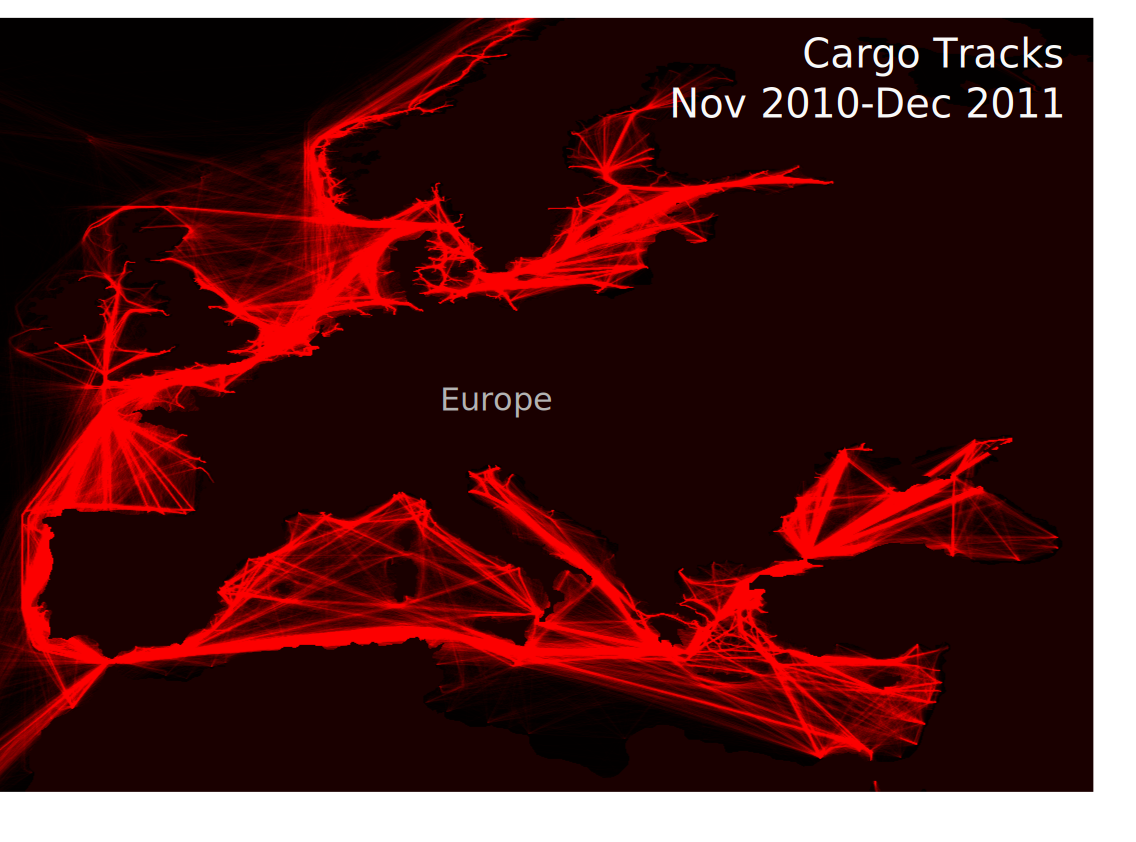
\includegraphics[width=140mm]{figures/cargo-lanes-eu-red-labeled.pdf}
  \caption[Cargo density, Europe]{Cargo density grid, generated by combining AIS and VOS records.}
  \label{fig:eu-cargo-density}
\end{figure}


\subsection{Speed}

\begin{figure}
  \centering
  \hspace*{-0.2in}
  \includegraphics[width=160mm]{figures/speed-boxplot.pdf}
  \caption[Validated ship speeds by class]{Boxplot of validated ship speeds by class.}
  \label{fig:vessel-speed-boxplot} % TODO Oliver: and? in theory I shouldn't have to read that part of the paper.
\end{figure}

Ship speed is an important indicator to answer a variety of questions, but is challenging to represent spatially. Ship speed is sensitive to the observation frequency at a particular location, and sensitive to accurate distance and time measurements, all three of which are needed to compute averaged velocities. The speed distribution of each vessel class was examined, through boxplots (Figure \ref{fig:vessel-speed-boxplot}) and kernel density estimation (Figure \ref{fig:vessel-speed-density}). The density estimation shows that for many vessel classes, distinct speed patterns exist. For example, support vessels, which include tugs and barges move much more slowly than high-speed transport vessels. Other classes are less distinct in speed signature: cargo and tanker vessels have surprisingly similar average speeds, though disaggregating the results spatially (Figure \ref{fig:speed-ship-map}) shows they have strong regional differences masked in the overall average.

% graphs of SHIP SPEED by type, either using kernel estimation or simple histograms depending on the clarity of the data.
\begin{figure}[t]
  \centering
  \hspace*{-0.2in}
  \includegraphics[width=165mm]{figures/speed-comparison-qqplot.pdf}
  \caption[Validated ship speeds by class, kernel density estimation]{Distribution of validated ship movement speeds, computed using kernel density comparisons, as described in \cite{bowman1997applied}.}
  \label{fig:vessel-speed-density}
\end{figure}

\begin{figure}[t]
  \centering
  \includegraphics[width=150mm]{figures/speed_map_labeled.pdf}
  \caption[Average ship speeds, North America and Europe]{Average ship speed examples. Scale shows 10-20 Kts/hr range for all vessels. Of note is the large difference in speeds between the opposite shores of North America.}
  \label{fig:speed-ship-map}
\end{figure}

\section{Uncertainty}

% XXX XXX section needs reworking.
AIS observations rely on terrestrial radio antennae to collect data, and their coverage of the near shore is incomplete. Many areas lack AIS observations, but are well-represented in the VOS data, showing data gaps. To account for this gap, I examined the coverage of the largest world ports, as identified in the World Port Index~\citep{worldportindex}. Of the large ports in the index, 112 of 155 (72.3\%) had 100 or more unique vessels, and of medium ports, 187 of 357 (52.4\%). The identified ports show concordance with the major ports identified in \cite{ducruet2012worldwide}. 

Individual vessel movement is also modeled simply, and barriers to movement are not accounted for, which can be important in areas with geographic and political features which limit movement. Future work should address this and other sources of uncertainty within the results.

% at a minimum, include our "obs per area" figure to show what kind of density we have, what \% of major world ports is sampled.
%- ports: of large ports in WPI, 112/155 (72.3\%) had 100 or more unique vessels, and 187/357 (52.4\%) of medium ports, we have AIS for much, but not all of the important near shore areas.

%mention the difficiencies of some areas (why are we routing some data through land masses?)

%Only have single average vessel speed
%Don't have detailed attributes for each segment.
% XXX Oliver: Why can't you calculate actual average speed using segment lengths?  Some jerk is going to ask. <- self-fulfilling



% XXX future work:

% ships by season? just static results here, can do some dynamic stuff later.
